%%%%%%%%%%%%%%
%% Run LaTeX on this file several times to get Table of Contents,
%% cross-references, and citations.

%% If you have font problems, you may edit the w-bookps.sty file
%% to customize the font names to match those on your system.

%% w-bksamp.tex. Current Version: Feb 16, 2012
%%%%%%%%%%%%%%%%%%%%%%%%%%%%%%%%%%%%%%%%%%%%%%%%%%%%%%%%%%%%%%%%
%
%  Sample file for
%  Wiley Book Style, Design No.: SD 001B, 7x10
%  Wiley Book Style, Design No.: SD 004B, 6x9
%
%
%  Prepared by Amy Hendrickson, TeXnology Inc.
%  http://www.texnology.com
%%%%%%%%%%%%%%%%%%%%%%%%%%%%%%%%%%%%%%%%%%%%%%%%%%%%%%%%%%%%%%%%

%%%%%%%%%%%%%
% 7x10
%\documentclass{wileySev}

% 6x9
\documentclass{wileySix}

\usepackage{graphicx}
\usepackage{listings}

\usepackage{color}
 
\definecolor{codegreen}{rgb}{0,0.6,0}
\definecolor{codegray}{rgb}{0.5,0.5,0.5}
\definecolor{codepurple}{rgb}{0.58,0,0.82}
\definecolor{backcolour}{rgb}{0.95,0.95,0.92}
 
\lstdefinestyle{mystyle}{
    backgroundcolor=\color{backcolour},   
    commentstyle=\color{codegreen},
    keywordstyle=\color{magenta},
    numberstyle=\tiny\color{codegray},
    stringstyle=\color{codepurple},
    basicstyle=\footnotesize,
    breakatwhitespace=false,         
    breaklines=true,                 
    captionpos=b,                    
    keepspaces=true,                 
    numbers=left,                    
    numbersep=5pt,                  
    showspaces=false,                
    showstringspaces=false,
    showtabs=false,                  
    tabsize=2,
    language=sh
}
 
\lstset{style=mystyle}

%%%%%%%
%% for times math: However, this package disables bold math (!)
%% \mathbf{x} will still work, but you will not have bold math
%% in section heads or chapter titles. If you don't use math
%% in those environments, mathptmx might be a good choice.

% \usepackage{mathptmx}

% For PostScript text
\usepackage{w-bookps}

%%%%%%%%%%%%%%%%%%%%%%%%%%%%%%%%%%%%%%%%%%%%%%%%%%%%%%%%%%%%%%%%
%% Other packages you might want to use:

% for chapter bibliography made with BibTeX
% \usepackage{chapterbib}

% for multiple indices
% \usepackage{multind}

% for answers to problems
% \usepackage{answers}

%%%%%%%%%%%%%%%%%%%%%%%%%%%%%%
%% Change options here if you want:
%%
%% How many levels of section head would you like numbered?
%% 0= no section numbers, 1= section, 2= subsection, 3= subsubsection
%%==>>
\setcounter{secnumdepth}{3}

%% How many levels of section head would you like to appear in the
%% Table of Contents?
%% 0= chapter titles, 1= section titles, 2= subsection titles, 
%% 3= subsubsection titles.
%%==>>
\setcounter{tocdepth}{2}

%% Cropmarks? good for final page makeup
%% \docropmarks

%%%%%%%%%%%%%%%%%%%%%%%%%%%%%%
%
% DRAFT
%
% Uncomment to get double spacing between lines, current date and time
% printed at bottom of page.
% \draft
% (If you want to keep tables from becoming double spaced also uncomment
% this):
% \renewcommand{\arraystretch}{0.6}
%%%%%%%%%%%%%%%%%%%%%%%%%%%%%%

%%%%%%% Demo of section head containing sample macro:
%% To get a macro to expand correctly in a section head, with upper and
%% lower case math, put the definition and set the box 
%% before \begin{document}, so that when it appears in the 
%% table of contents it will also work:

\newcommand{\VT}[1]{\ensuremath{{V_{T#1}}}}

%% use a box to expand the macro before we put it into the section head:

\newbox\sectsavebox
\setbox\sectsavebox=\hbox{\boldmath\VT{xyz}}

%%%%%%%%%%%%%%%%% End Demo


\begin{document}


\booktitle{Cerdas Menguasai Phyton}
\subtitle{Dalam 24 Jam}

\authors{Rolly M. Awangga\\
\affil{Informatics Research Center}
%Floyd J. Fowler, Jr.\\
%\affil{University of New Mexico}
}

\offprintinfo{Cerdas Menguasai Git, First Edition}{Rolly M. Awangga}

%% Can use \\ if title, and edition are too wide, ie,
%% \offprintinfo{Survey Methodology,\\ Second Edition}{Robert M. Groves}

%%%%%%%%%%%%%%%%%%%%%%%%%%%%%%
%% 
\halftitlepage

\titlepage


\begin{copyrightpage}{2019}
%Survey Methodology / Robert M. Groves . . . [et al.].
%\       p. cm.---(Wiley series in survey methodology)
%\    ``Wiley-Interscience."
%\    Includes bibliographical references and index.
%\    ISBN 0-471-48348-6 (pbk.)
%\    1. Surveys---Methodology.  2. Social 
%\  sciences---Research---Statistical methods.  I. Groves, Robert M.  II. %
%Series.\\
%
%HA31.2.S873 2007
%001.4'33---dc22                                             2004044064
\end{copyrightpage}

\dedication{`Jika Kamu tidak dapat menahan lelahnya belajar, 
Maka kamu harus sanggup menahan perihnya Kebodohan.'
~Imam Syafi'i~}

\begin{contributors}
\name{Rolly Maulana Awangga,} Informatics Research Center., Politeknik Pos Indonesia, Bandung,
Indonesia



\end{contributors}

\contentsinbrief
\tableofcontents
\listoffigures
\listoftables
\lstlistoflistings


\begin{foreword}
Sepatah kata dari Kaprodi, Kabag Kemahasiswaan dan Mahasiswa
\end{foreword}

\begin{preface}
Buku ini diciptakan bagi yang awam dengan git sekalipun.

\prefaceauthor{R. M. Awangga}
\where{Bandung, Jawa Barat\\
Februari, 2019}
\end{preface}


\begin{acknowledgments}
Terima kasih atas semua masukan dari para mahasiswa agar bisa membuat buku ini 
lebih baik dan lebih mudah dimengerti.

Terima kasih ini juga ditujukan khusus untuk team IRC yang 
telah fokus untuk belajar dan memahami bagaimana buku ini mendampingi proses 
Intership.
\authorinitials{R. M. A.}
\end{acknowledgments}

\begin{acronyms}
\acro{ACGIH}{American Conference of Governmental Industrial Hygienists}
\acro{AEC}{Atomic Energy Commission}
\acro{OSHA}{Occupational Health and Safety Commission}
\acro{SAMA}{Scientific Apparatus Makers Association}
\end{acronyms}

\begin{glossary}
\term{git}Merupakan manajemen sumber kode yang dibuat oleh linus torvald.

\term{bash}Merupakan bahasa sistem operasi berbasiskan *NIX.

\term{linux}Sistem operasi berbasis sumber kode terbuka yang dibuat oleh Linus Torvald
\end{glossary}

\begin{symbols}
\term{A}Amplitude

\term{\hbox{\&}}Propositional logic symbol 

\term{a}Filter Coefficient

\bigskip

\term{\mathcal{B}}Number of Beats
\end{symbols}

\begin{introduction}

%% optional, but if you want to list author:

\introauthor{Rolly Maulana Awangga, S.T., M.T.}
{Informatics Research Center\\
Bandung, Jawa Barat, Indonesia}

Pada era disruptif  \index{disruptif}\index{disruptif!modern} 
saat ini. git merupakan sebuah kebutuhan dalam sebuah organisasi pengembangan perangkat lunak.
Buku ini diharapkan bisa menjadi penghantar para programmer, analis, IT Operation dan Project Manajer.
Dalam melakukan implementasi git pada diri dan organisasinya.

Rumusnya cuman sebagai contoh aja biar keren\cite{awangga2018sampeu}.

\begin{equation}
ABC {\cal DEF} \alpha\beta\Gamma\Delta\sum^{abc}_{def}
\end{equation}

\end{introduction}

%%%%%%%%%%%%%%%%%%Isi Buku_

\chapter{CHAPTER I}
\section{Python}
	\subsection{Background}
	\label{Background}
	\par
	Python adalah sebuah bahasa pemrograman yang bersifat interpreter, interactive, object-oriented, dan dapat beroperasi hampir pada semua platform seperti Windows, Linux, Mac. Python termasuk sebagai bahasa pemrograman yang dapat dengan mudah di pelajari karena sintaks yang jelas dan mudah dipahami, dan dapat dikombinasikan dengan penggunaan modul yang siap pakai, dan struktur data tingkat tinggi yang efisien \cite{prasetya2012deteksi}.
	\par
	Python memiliki kepustakaan atau biasa disebut library yang sangat luas, dan dalam distribusi Python yang telah disediakan, hal tersebut diakibatkan oleh pendistribusian Python yang bebas karena bahasa pemrograman Python merupakan bahasa pemrograman yang freeware atau bebas dalam hal pengembangannya. Python adalah sebuah bahasa pemrograman yang dapat dengan mudah dibaca dan terstruktur, hal tersebut dikarenakan penggunaan sistem identasi, yaitu pemisahan blok-blok program susunan identasi, jadi untuk menambahkan sub-sub program dalam sebuah blok program, sub program tersebut harus diletakkan pada satu atau lebih spasi dari kolom sebuah blok \cite{perkasa2014rancang}.
	\par
	Bahasa pemrograman Python dibuat oleh Guido Van Rossum. Dikarenakan para pengembang software atau perangkat lunak lebih cenderung memilih kecepatan dalam menyelesaikan suatu proyek dibandingkan dengan kecepatam proses dari program yang dijalankan, maka dari itu bahasa pemrograman Python dapat dibilang bahasa pemerograman yang kecepatannya dapat melebihi bahasa pemrograman C. Akan tetapi bahasa pemrograman Python lebih lambat dalam memproses suatu program dibandingkan bahasa pemrograman C. dengan berkembangnya kecepatan prosesor dan memori saat ini, mengakibatkan tidak terlihatnya keterlambatan dari sebuah program yang menggunakan bahasa pemrograman Python \cite{miftakhuddinimplementasi}.

	\subsection{Problems}
		\begin{itemize}
			\item Kurangnya pemahaman tentang bahasa pemrograman Python
			\item Kurang mengerti dalam hal fungsi-fungsi yang terdapat pada bahasa pemrograman Python
		\end{itemize}

	\subsection{Objective and Contribution}
		\subsubsection{Objective}
			\begin{itemize}
				\item Dapat memahami tentang bahasa pemrograman Python
				\item Dapat memahami fungsi fungsi yang terdapat pada bahasa pemrograman Python
			\end{itemize}
	
		\subsubsection{Contribution}
			\begin{itemize}
				\item Dapat membangun sebuah sistem dengan menggunakan bahasa pemrograman Python
				\item Dapat membangun sebuah alat yang berguna, menggunakan mikrokontroler dan bahasa pemrograman python
			\end{itemize}

	\subsection{Scoop and Environtment}
		\begin{itemize}
			\item Pengenanalan tentang bahasa pemrograman Python
			\item Pengenalan fungsi-fungsi yang terdapat pada bahasa pemrograman Python
		\end{itemize}


\chapter{CHAPTER II}

\subsection{Teori}
\begin{enumerate}
\item Pada python variabel tidak perlu dideklarasikan, pendeklarasian terjadi secara otomatis pada saat memberikan suatu nilai atau data ke variabel. Terdapat beberapa jenis tipe data variabel pada python, diantaranya :
				\begin{itemize}
\item Python Numbers, dimana akan menyimpan data yang berupa angka. Penggunaan pada python sebagai berikut : 
					\begin{lstlisting}
					var1 = 5
					var2 = 48.9
					\end{lstlisting}
	
\item Python Text, dimana akan menyimpan data yang berupa teks ataupun karakter. Penggunaan pada python harus diapitkan oleh tanda petik ("..."), contohnya :
					\begin{lstlisting}
					nama = "Irvan"
					jnskelamin = "L"
					\end{lstlisting}
					
\item Python Boolean, dimana yang hanya memiliki 2 nilai yaitu True dan False saja. penggunaan pada python huruf pertama harus kapital, contohnya :
					\begin{lstlisting}
					var3 = True
					var4 = False
					\end{lstlisting}
				\end{itemize}

			\item \begin{itemize}
					\item Meminta input pada user
					nama = input("Masukkan Nama Anda : ")
					
					\item menampilkan output
					print "Hello Nama Saya Adalah",nama
				\end{itemize}

			\item \begin{itemize}
					\item Operator tambah
					\begin{lstlisting}
					a = b + c
					\end{lstlisting}

					\item Operator kurang
					\begin{lstlisting}
					a = b - c
					\end{lstlisting}

					\item Operator kali
					\begin{lstlisting}
					a = b * c
					\end{lstlisting}

					\item Operator bagi
					\begin{lstlisting}
					a = b / c
					\end{lstlisting}

					\item Konversi integer ke string
					\begin{lstlisting}
					konvVar = str(var1)
					\end{lstlisting}

					\item Konversi string ke integer
					\begin{lstlisting}
					konvVar = int(var2)
					\end{lstlisting}
				\end{itemize}

			\item \begin{itemize}
				\item Pengulangan for, kemampuan mengulang proses data menggunakan urutan apapun, seperti list.
				contoh penggunaan pada Python dan contoh kode adalah :

					\begin{lstlisting}
					for i in range(10):
						print(i)
					\end{lstlisting}
					
				\item Pengulangan while, kemampuan mengulang proses data yang akan terus berlanjut jika kondisinya True.
				contoh penggunaan pada Python dan contoh kode adalah :
					\begin{lstlisting}
					i= 0
					while i < 10 :
						i=i+1
						print ("loop ke =", i)
					\end{lstlisting}
				\end{itemize}
				
			\item Pengambilan keputusan berguna untuk menentukan tindakan apa yang akan diambil sesuai dengan kondisi yang ada. Contohnya :
				\begin{lstlisting}
				nilai = 9
				if(nilai > 7):
					print("Selamat Anda Lulus")
				else:
					print("Maaf Anda Tidak Lulus")
				\end{lstlisting}
				
				Dan untuk kondisi di dalam kondisi contohnya :
				
				\begin{lstlisting}
				gaji = 10000000
				berkeluarga = True
				if gaji > 3000000:
					print "Gaji sudah diatas UMR"
					if berkeluarga:
							print "Wajib ikutan asuransi dan menabung untuk pensiun"
						else:
							print "Tidak perlu ikutan asuransi"
				else:
					print "Gaji belum UMR"
				\end{lstlisting}

			\item \begin{itemize}
					\item Syntax Errors, Salahnya dalam penulisan sintaks.
					cara penanganannya adalah dengan menganalisa bagian kode yang error dan memperbaiki sintaks tersebut.
					
					\item Exceptions, error yang terjadi karena sintaks tidak dapat dieksekusi.
					cara penanganannya adalah dengan menganalisa bagian kode yang error dan memperbaiki sintaks tersebut.
				\end{itemize}
			
			\item Try Except adalah cara penanganan error pada Python.
			Contohnya : 
				\begin{lstlisting}
				x = 0
				try:
					x = 1 / 0
				except Exception, e:
					print e
				\end{lstlisting}

		\end{enumerate}
		
	\subsection{Keterampilan Pemrograman}
		\begin{enumerate}
			\item \lstinputlisting{src/chapter2/1174043_1.py}

			\item \lstinputlisting{src/chapter2/1174043_2.py}

			\item \lstinputlisting{src/chapter2/1174043_3.py}

			\item \lstinputlisting{src/chapter2/1174043_4.py}

			\item \lstinputlisting{src/chapter2/1174043_5.py}

			\item \lstinputlisting{src/chapter2/1174043_6.py}

			\item \lstinputlisting{src/chapter2/1174043_7.py}

			\item \lstinputlisting{src/chapter2/1174043_8.py}

			\item \lstinputlisting{src/chapter2/1174043_9.py}

			\item \lstinputlisting{src/chapter2/1174043_10.py}
			
			\item \lstinputlisting{src/chapter2/1174043_11.py}
		\end{enumerate}
		
	\subsection{Keterampilan Penanganan Error}
		\begin{enumerate}
			\item TypeError yaitu error di dalam tipe data disaat melakukan substring dan ingin memasukkannya ke dalam kondisi for 
			yang hanya menerima tipe int. jadi harus merubah tipe inputan yaitu string menjadi integer.

			\item \lstinputlisting{src/chapter2/1174043_2err.py}
		\end{enumerate}

\chapter{CHAPTER III}
	\subsection{Pemahaman Teori}
		\begin{enumerate}
			\item	\begin{itemize}
						\item Fungsi adalah bagian dari program yang berupa blok kode yang diberikan nama dan nama tersebut berguna untuk memanggil fungsi tersebut.
					
						\item Inputan fungsi adalah sebuah fungsi yang telah di sediakan pada library python, yang berguna untuk menerima inputan dari user.
					
						\item Kembalian fungsi adalah sebuah nilai balikan yang diberikan oleh sebuah fungsi yang dibuat.
					\end{itemize}
					
					Contoh Program : 
					\lstinputlisting[language=Python, firstline=2, lastline=8]{src/chapter3/teori_1174043_chap3.py}
					
			\item paket adalah sebuah cara yang dilakukan untuk memanggil file script python, yang nantinya akan digunakan fungsi fungsi yang terdapat pada file script yang dipanggil tersebut. cara pemanggilan paket dengan cara :
				\begin{verbatim}
				import scriptFilePython
				\end{verbatim}
			
			Contoh Program :
			\lstinputlisting[language=Python, firstline=11, lastline=11]{src/chapter3/teori_1174043_chap3.py}
			
			\item	\begin{itemize}
						\item Kelas merupakan sebuah cetakan atau Blueprint yang berguna untuk mencetak objek.
						
						\item Objek merupakan sebuah objek yang dari proses hasil dari cetakan atau blueprint.
						
						\item Atribut merupakan penggambaran data yang bisa memberikan sebuah informasi kelas atau objek dimana atribut tersebut berada.
						
						\item Method merupakan fungsi atau prosedur yang bergabung dengan sebuah objek dan juga atribut.
					\end{itemize}
					
					Contoh Program :
					\lstinputlisting[language=Python, firstline=14, lastline=17]{src/chapter3/teori_1174043_chap3.py}
					
			\item cara pemanggilan library kelas dari instansiasi, adalah dengan cara mengubah library kelas yang dipanggil menjadi sebuah objek.
			
			Contoh Program : 
			\lstinputlisting[language=Python, firstline=22, lastline=24]{src/chapter3/teori_1174043_chap3.py}
			
			\item Jadi pemakaian paket dengan perintah from kalkulator import penambahan berguna untuk menghemat memori pemakaian pada program, karena hanya memanggil fungsi yang diperlukan saja pada library yang terpanggil. cara memanggilnya dengan cara :
				\begin{verbatim}
				from scripFilePython import namaFungsi, namaFungsi2
				\end{verbatim}
				
			Contoh Program :
			\lstinputlisting[language=Python, firstline=27, lastline=27]{src/chapter3/teori_1174043_chap3.py}
			
			\item \lstinputlisting[language=Python, firstline=30, lastline=35]{src/chapter3/teori_1174043_chap3.py}
			
			\item \lstinputlisting[language=Python, firstline=38, lastline=42]{src/chapter3/teori_1174043_chap3.py}
			
		\end{enumerate}
		
	\subsection{Keterampilan Pemrograman}
		\begin{enumerate}
			\item Jawaban soal no 1
				\lstinputlisting{src/chapter3/chap3_1174043_no1.py}
				
				\begin{figure} [ht]
					\centerline{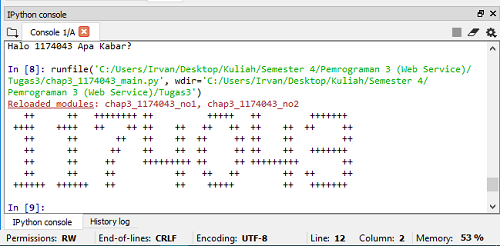
\includegraphics[width=0.6\textwidth]{figures/chapter3/1_1174043.png}}
					\caption{Jawaban No. 1}
					\label{1}
				\end{figure}

				\ref{1_1174043}
				
			\item Jawaban soal no 2
				\lstinputlisting{src/chapter3/chap3_1174043_no2.py}
				
				\begin{figure} [ht]
					\centerline{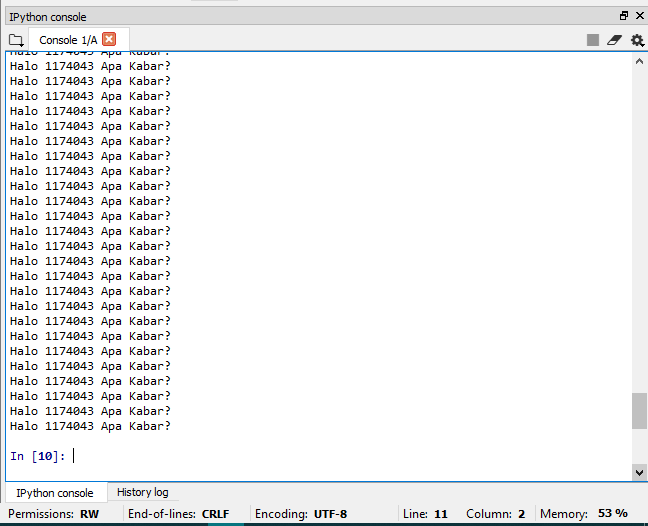
\includegraphics[width=1\textwidth]{figures/chapter3/2_1174043.png}}
					\caption{Jawaban No. 2}
					\label{2}
				\end{figure}

				\ref{2_1174043}
			
			\item Jawaban soal no 3
				\lstinputlisting{src/chapter3/chap3_1174043_no3.py}
				
				\begin{figure} [ht]
					\centerline{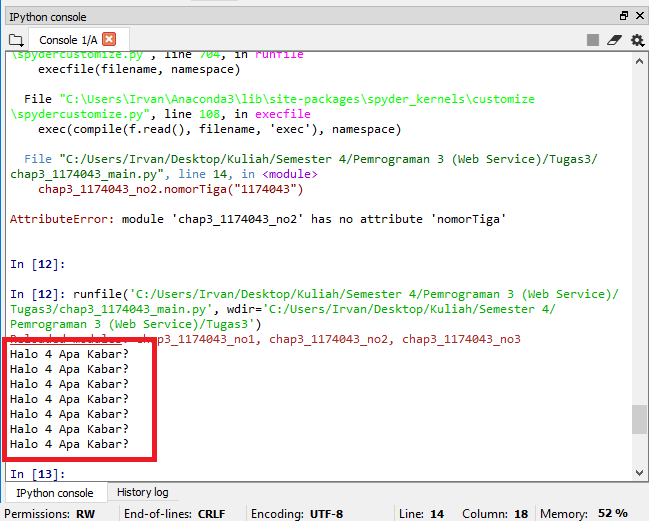
\includegraphics[width=1\textwidth]{figures/chapter3/3_1174043.png}}
					\caption{Jawaban No. 3}
					\label{3}
				\end{figure}

				\ref{3_1174043}
				
			\item Jawaban soal no 4
				\lstinputlisting{src/chapter3/chap3_1174043_no4.py}
				
				\begin{figure} [ht]
					\centerline{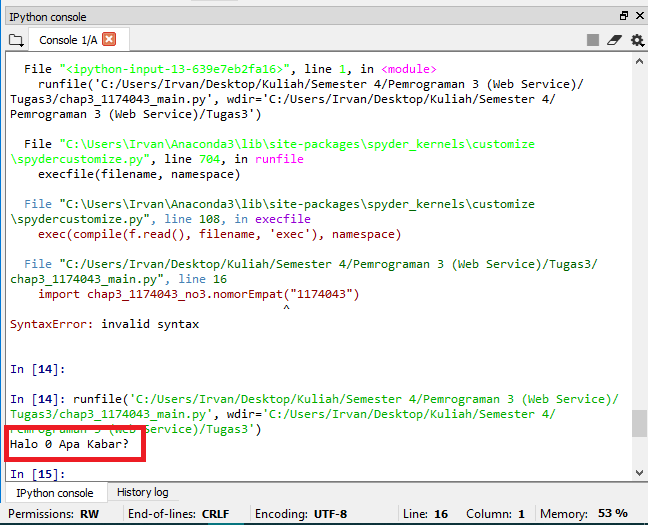
\includegraphics[width=1\textwidth]{figures/chapter3/4_1174043.png}}
					\caption{Jawaban No. 4}
					\label{4}
				\end{figure}

				\ref{4_1174043}
				
			\item Jawaban soal no 5
				\lstinputlisting{src/chapter3/chap3_1174043_no5.py}
				
				\begin{figure} [ht]
					\centerline{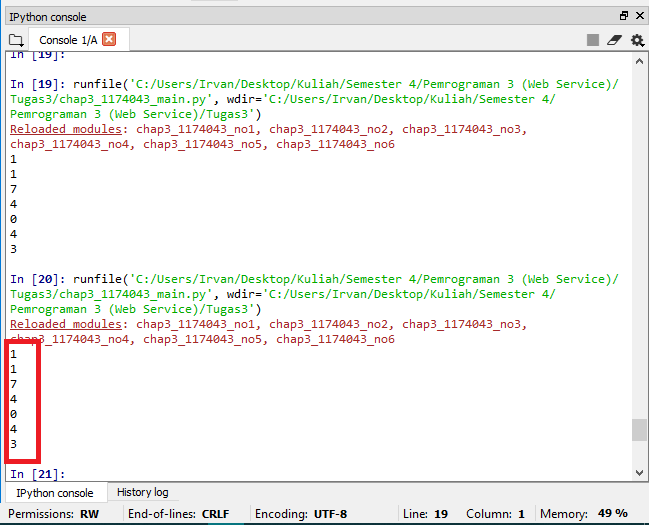
\includegraphics[width=1\textwidth]{figures/chapter3/5_1174043.png}}
					\caption{Jawaban No. 5}
					\label{5}
				\end{figure}

				\ref{5_1174043}
				
			\item Jawaban soal no 6
				\lstinputlisting{src/chapter3/chap3_1174043_no6.py}
				
				\begin{figure} [ht]
					\centerline{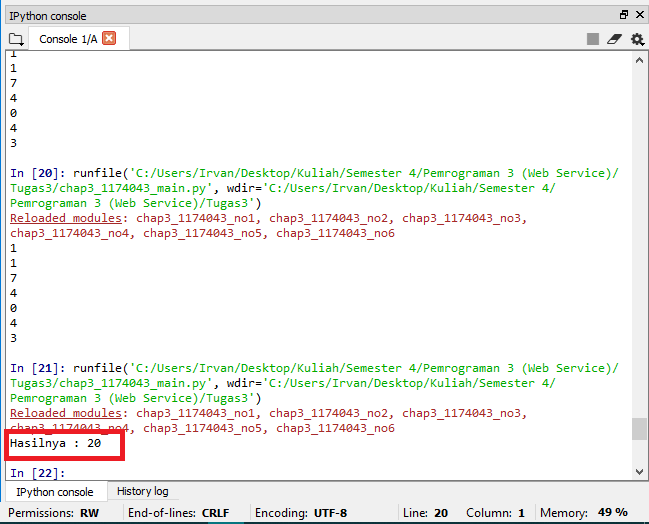
\includegraphics[width=1\textwidth]{figures/chapter3/6_1174043.png}}
					\caption{Jawaban No. 6}
					\label{6}
				\end{figure}

				\ref{6_1174043}
				
			\item Jawaban soal no 7
				\lstinputlisting{src/chapter3/chap3_1174043_no7.py}
				
				\begin{figure} [ht]
					\centerline{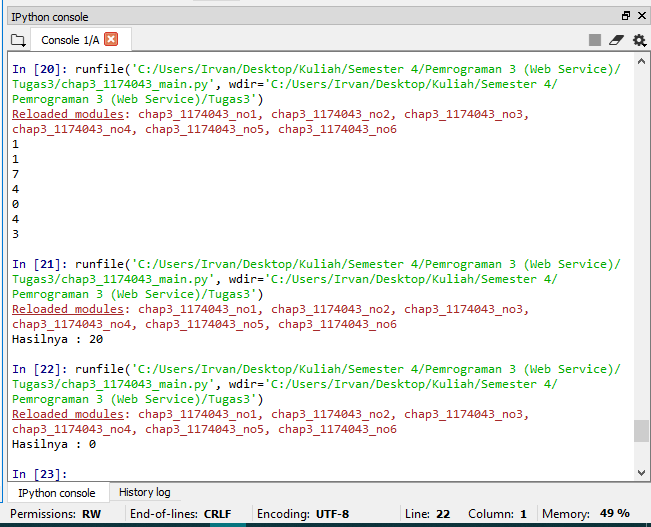
\includegraphics[width=1\textwidth]{figures/chapter3/7_1174043.png}}
					\caption{Jawaban No. 7}
					\label{7}
				\end{figure}

				\ref{7_1174043}
				
			\item Jawaban soal no 8
				\lstinputlisting{src/chapter3/chap3_1174043_no8.py}
				
				\begin{figure} [ht]
					\centerline{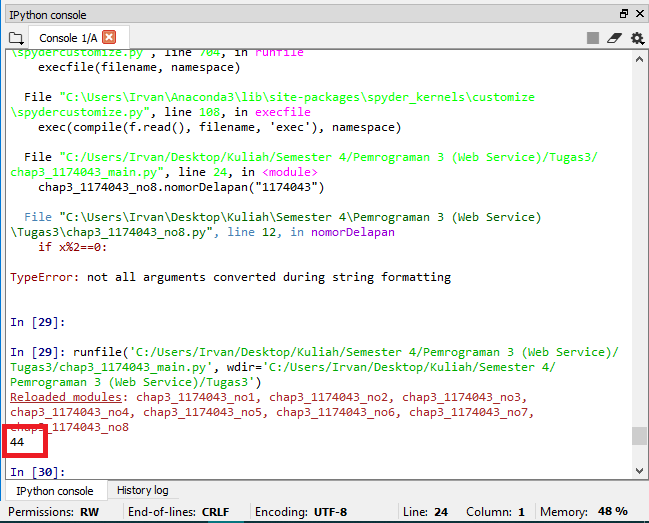
\includegraphics[width=1\textwidth]{figures/chapter3/8_1174043.png}}
					\caption{Jawaban No. 8}
					\label{8}
				\end{figure}

				\ref{8_1174043}
				
			\item Jawaban soal no 9
				\lstinputlisting{src/chapter3/chap3_1174043_no9.py}
				
				\begin{figure} [ht]
					\centerline{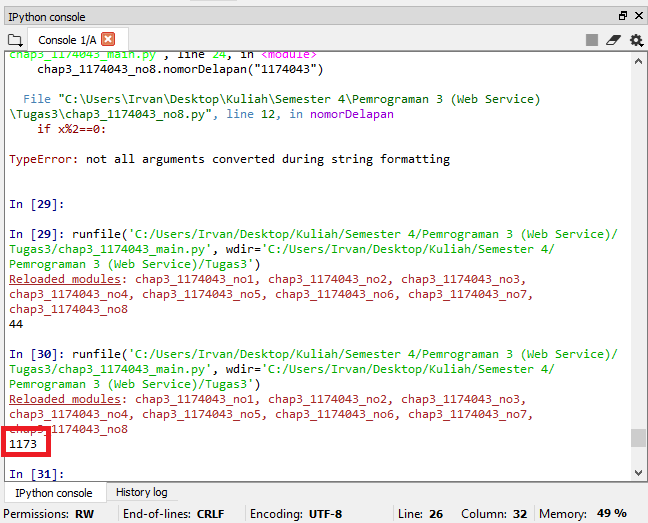
\includegraphics[width=1\textwidth]{figures/chapter3/9_1174043.png}}
					\caption{Jawaban No. 9}
					\label{9}
				\end{figure}

				\ref{9_1174043}
				
			\item Jawaban soal no 10
				\lstinputlisting{src/chapter3/chap3_1174043_no10.py}
				
				\begin{figure} [ht]
					\centerline{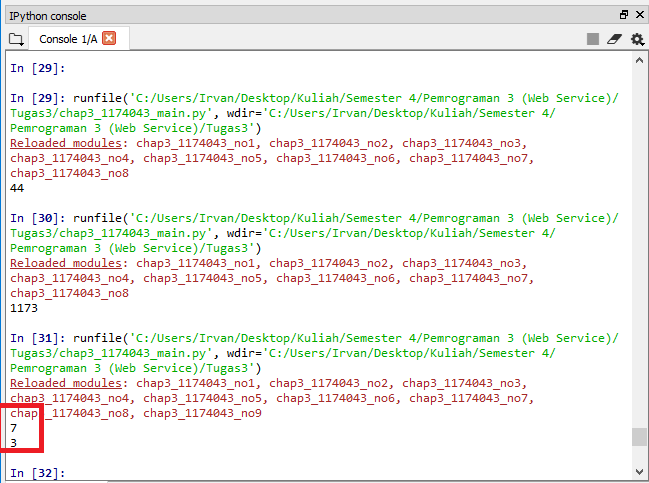
\includegraphics[width=1\textwidth]{figures/chapter3/10_1174043.png}}
					\caption{Jawaban No. 10}
					\label{10}
				\end{figure}

				\ref{10_1174043}
				
			\item Jawaban soal no 11
			
				File 3lib.py
				\lstinputlisting{src/chapter3/chap3_1174043_3lib.py}
				
				File main.py
				\lstinputlisting{src/chapter3/chap3_1174043_main.py}
				
				\begin{figure} [ht]
					\centerline{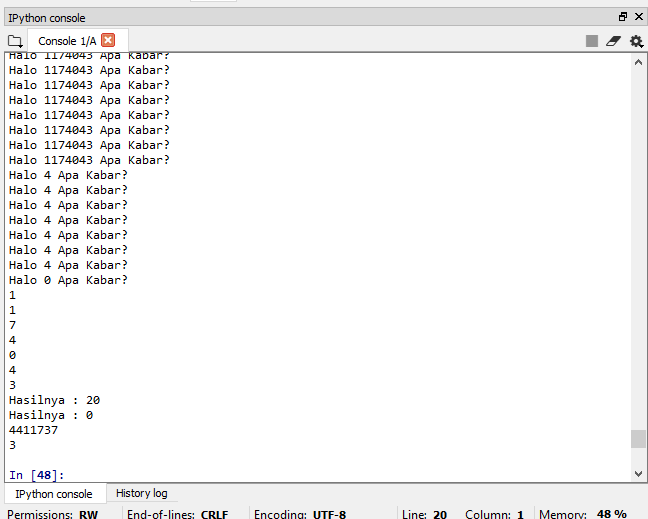
\includegraphics[width=1\textwidth]{figures/chapter3/11_1174043.png}}
					\caption{Jawaban No. 11}
					\label{11}
				\end{figure}

				\ref{11_1174043}
				
			\item Jawaban soal no 12
			\lstinputlisting{src/chapter3/chap3_1174043_kelas3lib.py}
		
		\end{enumerate}
		
		\subsection{Keterampilan Penanganan Error}
			\begin{enumerate}
				\item \lstinputlisting{src/chapter3/chap3_1174043_3err.py}
			
			\end{enumerate}
			
		



\bibliographystyle{IEEEtran} 
%\def\bibfont{\normalsize}
\bibliography{references}


%%%%%%%%%%%%%%%
%%  The default LaTeX Index
%%  Don't need to add any commands before \begin{document}
\printindex

%%%% Making an index
%% 
%% 1. Make index entries, don't leave any spaces so that they
%% will be sorted correctly.
%% 
%% \index{term}
%% \index{term!subterm}
%% \index{term!subterm!subsubterm}
%% 
%% 2. Run LaTeX several times to produce <filename>.idx
%% 
%% 3. On command line, type  makeindx <filename> which
%% will produce <filename>.ind 
%% 
%% 4. Type \printindex to make the index appear in your book.
%% 
%% 5. If you would like to edit <filename>.ind 
%% you may do so. See docs.pdf for more information.
%% 
%%%%%%%%%%%%%%%%%%%%%%%%%%%%%%

%%%%%%%%%%%%%% Making Multiple Indices %%%%%%%%%%%%%%%%
%% 1. 
%% \usepackage{multind}
%% \makeindex{book}
%% \makeindex{authors}
%% \begin{document}
%% 
%% 2.
%% % add index terms to your book, ie,
%% \index{book}{A term to go to the topic index}
%% \index{authors}{Put this author in the author index}
%% 
%% \index{book}{Cows}
%% \index{book}{Cows!Jersey}
%% \index{book}{Cows!Jersey!Brown}
%% 
%% \index{author}{Douglas Adams}
%% \index{author}{Boethius}
%% \index{author}{Mark Twain}
%% 
%% 3. On command line type 
%% makeindex topic 
%% makeindex authors
%% 
%% 4.
%% this is a Wiley command to make the indices print:
%% \multiprintindex{book}{Topic index}
%% \multiprintindex{authors}{Author index}

\end{document}

